\documentclass[../main.tex]{subfiles}
\graphicspath{{\subfix{../figures/}}}
%
\begin{document}
\section{命令模式(Command)}
命令(Command)模式属于对象的行为模式。命令模式又称为行动(Action)模式或事务(Transaction)模式。
命令模式是对命令的封装。命令模式把发出命令的责任和执行命令的责任分割开,委派给不同的对象。
每一个命令都是一个操作:请求的一方发出请求要求执行一个操作;接收的一方收到请求,并执行操作。命令模式允许请求的一方和接收的一方独立开来,使得请求的一方不必知道接收请求的一方的接口,更不必知道请求是怎么被接收,以及操作是否被执行,何时被执行,以及是怎么被执行的。

\subsection{命令模式的结构}
\textbf{命令模式的类图}:下面以一个示意性的系统为例,说明命令模式的结构。
%
\begin{figure}[H]
  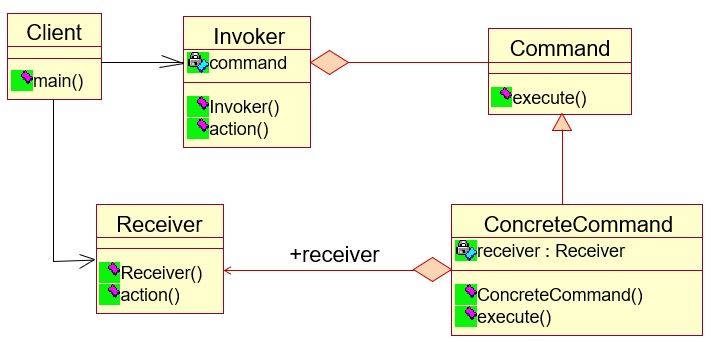
\includegraphics[width=0.55\textwidth]{30_1.jpg}
\end{figure}
%
\textbf{命令模式涉及到5个角色}:
\begin{itemize}
  \item 客户端(Client)角色:创建了一个具体命令(ConcreteCommand)对象并确定其接收者。
  \item 命令角色(Command):声明了一个给所有具体命令类的抽象接口。
  \item 具体命令(ConcreteCommand)角色:定义一个接收者和行为之间的弱偶合;实现execute()方法,负责调用接收者的相应操作。execute()方法通常叫做执行方法。
  \item 请求者(Invoker)角色:负责发出一个请求。
  \item 接收者(Receiver)角色:任何一个类都可以成为接收者;实施和执行请求的方法叫做行动方法。
\end{itemize}
%
\lstinputlisting[language=java]{./code/30/1/Invoker.java}
%
Receiver类是命令的接收者,在命令的控制下执行行动方法。这里仅给出一个action()方法的示意性实现。代码如下:
%
\lstinputlisting[language=java]{./code/30/1/Receiver.java}
\lstinputlisting[language=java]{./code/30/1/Command.java}
\lstinputlisting[language=java]{./code/30/1/ConcreteCommand.java}
\lstinputlisting[language=java]{./code/30/1/Client.java}
%
命令模式的活动序列:
%
\begin{figure}[H]
  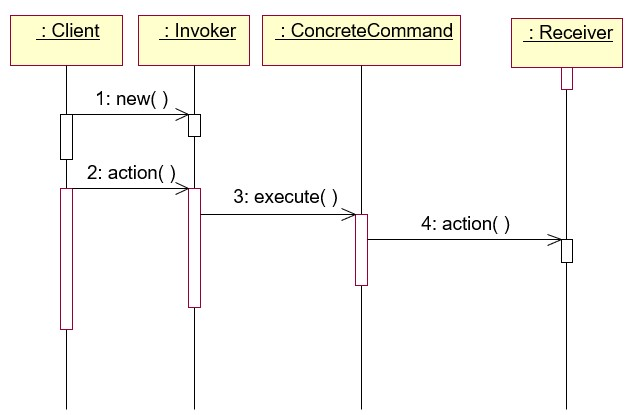
\includegraphics[width=0.45\textwidth]{30_2.jpg}
\end{figure}
%
\subsection{命令模式的优劣}
\begin{itemize}
  \item 优点:
    \begin{enumerate}
      \item 命令模式把请求一个操作的对象与知道怎么执行一个操作的对象分割开。
      \item 命令类与其他任何别的类一样,可以修改和扩展。
      \item 可以把命令对象聚合在一起,合成为合成命令。比如上面的例子里所讨论的宏命令便是合成命令的例子。合成命令是合成模式的应用。
      \item 由于加进新的具体命令类不影响其他的类,因此增加新的具体命令类很容易。
    \end{enumerate}
  \item 缺点:
    使用命令模式会导致某些系统有过多的具体命令类。某些系统可能需要几十个,几百个甚至几千个具体命令类,这会使命令模式在这样的系统里变得不实际。
\end{itemize}
%
\subsection{例:AudioPlayer 系统}
\noindent \textbf{系统的描述}:
User有一个录音机,该录音机有play、rewind和stop功能,录音机的键盘是请求者角色(Invoker), User是客户端类,录音机是接收者角色。Command类是抽象命令角色,PlayCommand、StopCommand和RewindCommand是具体命令类。
User不需要知道play、rewind和stop功能是怎么执行的,这些命令执行的细节由键盘Keypad具体实施。
User只需要在键盘上按下相应的键就行了。

\textbf{系统的角色}:
\begin{itemize}
  \item 客户端(Client)角色: User
  \item 请求者(Invoker)角色:Keypad
  \item 抽象命令(Command)角色:Command
  \item 具体命令角色:PlayCommand、RewindCommand、StopCommand
  \item 接收者角色:录音机AudioPlayer
\end{itemize}
%
请求者Invoker角色Keypad源代码:
%
\lstinputlisting[language=java]{./code/30/2/Keypad.java}
%
抽象命令角色Command源代码:
%
\lstinputlisting[language=java]{./code/30/2/Command.java}
%
具体命令类PlayCommand源代码:
%
\lstinputlisting[language=java]{./code/30/2/PlayCommand.java}
%
具体命令类StopCommand源代码:
%
\lstinputlisting[language=java]{./code/30/2/StopCommand.java}
%
具体命令类RewindCommand源代码:
%
\lstinputlisting[language=java]{./code/30/2/RewindCommand.java}
%
接收者类AudioPlayer源代码:
%
\lstinputlisting[language=java]{./code/30/2/AudioPlayer.java}
\lstinputlisting[language=java]{./code/30/2/User.java}
%
系统的时序图如下:
%
\begin{figure}[H]
  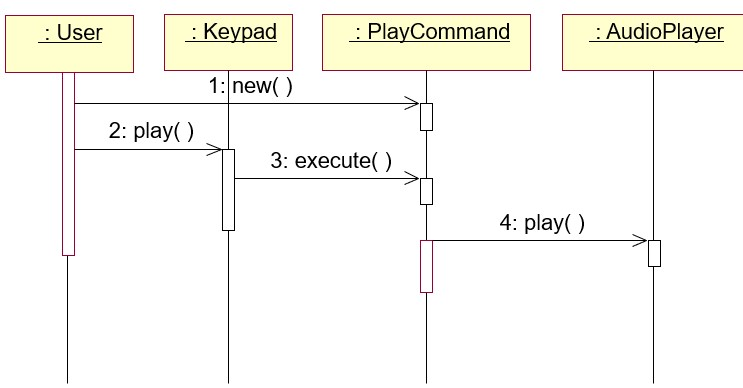
\includegraphics[width=0.55\textwidth]{30_3.jpg}
\end{figure}
%
\textbf{增加宏命令功能}:
设想User的录音机有一个记录功能,可以把每一次执行的命令记录下来,再在任何需要的的时候重新把这些记录下来的命令一次性执行,这就是所谓的宏命令集功能。因此,User的录音机系统现在有四个键,分别为播音,倒带,停止和宏命令功能。此时系统的设计与前面的设计相比有所增强,主要体现在User类现在有了一个新的方法,用以操作宏命令键。
带有宏命令集功能的录音机模拟系统的设计图如下:
%
\begin{figure}[H]
  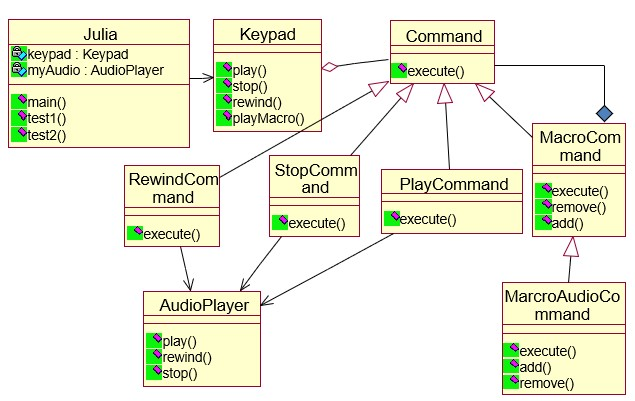
\includegraphics[width=0.55\textwidth]{30_4.jpg}
\end{figure}
%
\lstinputlisting[language=java]{./code/30/2/MacroCommand.java}
%
具体宏命令MacroAudioCommand类负责把个别的命令合成宏,代码如下:
%
\lstinputlisting[language=java]{./code/30/2/MacroAudioCommand.java}
%
Julia类的方法test2()源代码如下:
\begin{lstlisting}[language=java]
public static void test2() {
  Command play=new PlayCommand(myAudio);
  Command stop=new PlayCommand(myAudio);
  Command rewind=new PlayCommand(myAudio);
  MacroCommand macro=new MacroCommand();
  macro.add(play);
  macro.add(stop);
  macro.add(rewind);
  macro.add(stop);
  macro.add(play);
  macro.add(stop);
  KeyPad keypad=new KeyPad(play,stop,rewind,macro);
  keypad.playMacro();
}
\end{lstlisting}
%
\end{document}
